\section{Introducción}
\label{ch:intro}
El $\mu$Arm es un brazo robótico creado por la compañía UFACTORY\footnote{\url{https://www.ufactory.cc/\#/en/uarmswift}} el cual se ha diseñado con propósito principalmente didáctico.

En la actualidad, se puede obtener uno a través de su página web o de proveedores externos, pero no está previsto fabricar más, por lo que en un tiempo estará fuera de existencias.

Debido a su propósito didáctico, todos los recursos sobre el manipulador son de código libre, por lo que resultan accesibles a cualquiera que los necesite. Entre otros, se encuentran\footnote{todos los elementos descritos se encuentran disponibles tanto en \href{https://github.com/uArm-Developer}{GitHub} como en la web de \href{https://www.ufactory.cc/\#/en/support/download/pro}{UFACTORY}}:

\begin{itemize}
    \item \textit{Firmware} del $\mu$Arm Swift Pro.
    \item \ac{SDK} de Python para el $\mu$Arm Swift Pro.
    \item \textit{Firmware} que maneja el controlador del brazo.
    \item \ac{ROS} para el $\mu$Arm Swift Pro.
    \item Distintos ejemplos para toda la gama de brazos robóticos.
    \item \textit{$\mu$Arm Creator Studio}.
    \item Visión esquemática de las conexiones de la placa Arduino.
    \item Modelos 3D del brazo robótico.
    \item Guías de usuario, desarrollador y especificaciones técnicas.
\end{itemize}

Aprovechando dichos recursos, se pretende desarrollar un brazo robótico basado en el $\mu$Arm que esté impreso en 3D y sea controlado por un microcontrolador en conjunción con un ordenador cualquiera. Aprovechando los recursos provistos por UFACTORY, se busca que el brazo desarrollado sea más barato de construir (frente a los casi 800\euro{} que cuesta el original) y que pueda ser desarrollado por cualquiera con acceso a Internet y a los recursos necesarios, a saber, una impresora en 3D y un \ac{SW} de impresión en 3D.

\subsection{Propósito}
El propósito de este documento es establecer un punto de partida claro y conciso que permita empezar el desarrollo del brazo robótico sabiendo los puntos primordiales del mismo. A su vez, también pretende establecer ciertos puntos que se consideran importantes e incluso necesarios para poder continuar el desarrollo del sistema en un futuro, implementando nuevas funciones o arreglando errores que pudieran existir.

Este documento está dirigido a ingenieros que quieran llevar a cabo su propia implementación del brazo robótico o que quieran conocer la estructura en la que se basa el proyecto, así como las necesidades del mismo y las adiciones extraordinarias que se han incluido. A su vez, se pretende que sea accesible a cualquiera que pretenda iniciarse en el mundo de la robótica y que busque estudiar y aprender sobre el brazo robótico.

\subsection{Alcance}

El objetivo principal de este proyecto fin de grado es construir una brazo robótico similar al manipulador $\mu$Arm, al cual se le ha asignado el nombre \ac{pArm}.

Este brazo robótico debe ser capaz de moverse libremente dentro de su campo de movimiento, el cual está limitado por su estructura física. Además, el \pArm{} debe ser capaz de coger, transportar y depositar objetos de poco peso y, en consecuencia, debe ser capaz de describir trayectorias previamente planificadas o calculadas en el momento.

Es importante destacar que, dado que el brazo robótico \pArm{} no está sensorizado, este no será capaz de moverse de forma completamente autónoma ni de imitar movimientos realizados por el usuario.

Cabe destacar que el brazo robótico está controlado mediante un microcontrolador. Sin embargo, las instrucciones de movimiento y trayectorias no se computan, en principio, en el mismo sino en un ordenador auxiliar.

Debido a la estructura física, tamaño y materiales de fabricación, el \pArm{} no es un brazo robótico pensado para la realización de tareas industriales ni para el transporte de cargas pesadas.

En relación a lo anteriormente mencionado, la aplicación principal del \pArm{} es didáctica, dado que se busca construir un brazo robótico económico y sencillo que facilite la introducción de los usuarios a este tipo de tecnologías.


% \subsection{Definiciones, siglas, y abreviaturas}
% \begin{acronym}
    \acro{SDK}{\textit{Software Development Kit}}
    \acro{ROS}{\textit{Robot Operating System}}
    \acro{API}{\textit{Application Programming Interface}}
    \acro{SW}{\textit{software}}
    \acro{HW}{\textit{hardware}}
    \acro{pArm}{\textit{Printed -- Arm}}
    \acro{USB}{\textit{Universal Serial Bus}}
    \acro{ODS}{Objetivos de Desarrollo Sostenible}
    \acro{OS}{\textit{Open--Source}}
    \acro{OH}{\textit{Open--Hardware}}
    \acro{S1}{Sistema 1 -- ordenador}
    \acro{S2}{Sistema 2 -- \pArm{}}
    \acro{GUI}{\textit{Graphical User Interface}}
    \acro{GTK}{\textit{GIMP Toolkit}}
    \acro{SoC}{\textit{System On Chip}}
    \acro{PWM}{\textit{Pulse--Width Modulation}}
    \acro{GPIO}{\textit{General Purpose Input/Output}}
    \acro{UART}{\textit{Universal Asynchronous Receiver--Transmitter}}
    \acro{RAM}{\textit{Random Access Memory}}
    \acro{ADC}{\textit{Analog--Digital Conversor}}
    \acro{PLA}{Ácido Poliláctico}
    \acro{ABS}{Acrilonitrilo Butadieno Estireno}
    \acro{DSP}{\textit{Digital Signal Processor}}
    \acro{PLL}{\textit{Phase Loop Lock}}
    \acro{THT}{\textit{Through-Hole Technology}}
    \acro{SMD}{\textit{surface-mount device}}
    \acro{PCB}{\texit{Printed circuit board}}
    
\end{acronym}

\begin{itemize}
    \item \ac{SDK} -- colección de herramientas \ac{SW} disponibles para instalar en un único paquete.
    \item \textit{hand--shake} -- en informática, negociación entre pares para establecer de forma dinámica los parámetros de un canal de comunicaciones. 
    \item \ac{ROS} -- conjunto de librerías \ac{SW} que ayudan a construir aplicaciones para robots.
    \item \textit{Firmware} -- \ac{SW} programado que especifica el orden de ejecución del sistema.
    \item \ac{GUI} -- siglas que significan ``Interfaz Gráfica de Usuario'' (en castellano).
    \item \ac{GTK} -- biblioteca de componentes gráficos multiplataforma para desarrollar interfaces gráficas de usuario.
    \item \ac{SoC} -- tecnología de fabricación que integra todos o gran parte de los módulos en un circuito integrado. 
    \item \ac{PWM} -- Señal cuadrada de periodo habitualmente constante, entre flancos de subida, en la que se modula el tiempo a nivel alto
    \item \ac{GPIO} -- pin genérico cuyo comportamiento puede ser controlado en tiempo de ejecución.
    \item \ac{UART} -- estándar de comunicación dúplex.
    \item Dúplex -- término que define a un sistema que es capaz de mantener una comunicación bidireccional, enviando y recibiendo mensajes de forma simultánea.
    \item Widget -- la parte de una GUI (interfaz gráfica de usuario) que permite al usuario interconectar con la aplicación.
    \item \ac{RAM} -- memoria principal del ordenador, donde se guardan programas y datos, sobre la que se pueden efectuar operaciones de lectura y escritura.
    \item \textit{Deep--Sleep} -- estado de un microcontrolador en el cual consume muy poca cantidad de energía.
    \item \textit{bit} -- unidad mínima de información de un computador digital.
    \item \ac{THT} -- tecnología que utiliza agujeros pasantes que se practican en las placas de los circuitos impresos para el montaje de diferentes elementos electrónicos.
    \item \ac{SMD} -- tecnología que utiliza componentes de montaje superficial para la inserción de diferentes elementos electrónicos en un circuito impreso.
    \item \ac{PCB} -- Placa de circuito impreso.
\end{itemize}


\subsection{Visión global}
En las siguientes páginas se pasa a explicar los distintos detalles del sistema que debe construirse, respetándose la siguiente estructura:

\begin{itemize}
    \item Perspectiva del producto.
    \item Funciones del producto.
    \item Características del producto.
    \item Restricciones.
    \item Supuestos y dependencias.
    \item Requisitos propuestos.
\end{itemize}

En el punto ``Requisitos específicos'' (\ref{Requisitos específicos}) se detallan los requisitos específicos del sistema.

\section{Descripción general}
\label{Descripción general}

\subsection{Perspectiva del producto}
El \pArm{} se basa en el trabajo inicial del $\mu$Arm, no utilizando directamente lo desarrollado por la empresa UFACTORY sino aprovechando el trabajo ya realizado y los recursos disponibles para estudiarlos. Si bien es cierto que el $\mu$Arm ya es un sistema avanzado y capaz, como se explicó en la Introducción (\ref{ch:intro}), se pretende estudiar y desarrollar un sistema propio el cual pueda servir para ayudar y facilitar la entrada a este tipo de tecnologías a otras personas, haciéndolo comprensible y, aprovechando la tecnología de la impresión en 3D, fabricable por uno mismo.

Además, en relación a los \ac{ODS}, con el desarrollo de este sistema se pretende trabajar en:

\begin{itemize}
    \item [4 -] Educación de Calidad\footnote{\url{https://www.un.org/sustainabledevelopment/es/education/}}.
    \item [7 -] Energía Asequible y No Contaminante\footnote{\url{https://www.un.org/sustainabledevelopment/es/energy/}}.
    \item [10 -] Reducción de las desigualdades\footnote{\url{https://www.un.org/sustainabledevelopment/es/inequality/}}.
\end{itemize}

Para el primero, se tiene en cuenta que el producto se desarrollará siguiendo las iniciativas \ac{OS} y \ac{OH}, las cuales facilitan el acceso a la información a cualquiera que la requiera. Además, se facilitará el desarrollo al completo detallado y explicado, con la resolución de los problemas pertinentes y el porqué de ella.

Para el segundo, el \pArm{} utilizará la electricidad como fuente de energía, evitando así otras más contaminantes como las producidas por combustibles fósiles. En añadido, se trabajará para que el consumo de energía sea el menor posible, permitiendo así un mayor tiempo de uso con la misma fuente de alimentación y no abusando de los recursos de los que se disponen.

Finalmente, se pretende hacer que el \pArm{} tenga un coste bajo, permitiendo así el acceso a los recursos y los procesos de fabricación a todo el mundo que pudiera estar interesado y que disponga de la cantidad mínima necesaria para poder poner en funcionamiento el brazo robótico.

Por otra parte, el \pArm{} es dependiente de otro sistema que lo controle, ya que no se plantea como sistema autónomo. Por consiguiente, se proponen diversos métodos de conexión entre el brazo y dicho sistema. Por ejemplo, se puede utilizar el puerto serie \ac{USB} o bien comunicaciones inalámbricas, como \textit{Bluetooth} y \textit{WiFi}. Además, debido a su disponibilidad multiplataforma, se propone el uso de Python como alternativa de programación.

De ahora en adelante, se denominará ``\ac{S1}'' al equipo que controla al \pArm{}; y ``\ac{S2}'' al brazo robótico en sí.

Para este proyecto, se ha de desarrollar el \ac{SW} que se ejecutará en \ac{S1} y el \ac{SW} y el \ac{HW} que irán en \ac{S2}.
También habrá que adaptar la estructura mecánica para que esta pueda ser impresa en 3D.

\subsection{Interfaz del sistema}
En un principio, el sistema estará dividido en dos módulos:

\subsection*{\ac{S1}}
\ac{S1} consiste en un equipo el cual controlará el brazo robótico (\ac{S2}). Para ello, tal y como se planteó anteriormente, se propone como lenguaje de programación Python, el cual soporta la ejecución con \ac{GUI}.

En lo referente al sistema operativo, al ser una aplicación en Python la cual es multiplataforma, no se define ninguna restricción respecto al mismo.

Finalmente, se plantea la conexión con \ac{S2} utilizando el puerto serie \ac{USB}, por lo que también será necesario que el equipo anfitrión \ac{S1} disponga de una conexión de ese estilo.

En resumen (ver la tabla \ref{tab:s1_requirements}):

\begin{table}[H]
    \centering
    \begin{tabularx}{\textwidth}{| c | X | X |}
        \hline
        \textbf{Componente} & \textbf{Función} & \textbf{Restricciones} \\
        \hline\hline
        Sistema Operativo & Hospedar y ejecutar la aplicación Python que controlará el brazo robótico. & Debe poder ejecutar aplicaciones Python con \ac{GUI}, por ejemplo, \ac{GTK}. \\
        \hline
        \textit{Conexión con \ac{S2}} & Permitir la comunicación con el sistema \ac{S2} en modo dúplex. & Velocidad adaptable (\textit{baud--rate)} y capacidad para gran ancho de banda. \\
        \hline
        Python & Control del sistema \ac{S2} y monitorización del estado del mismo. & Versión Python $\geqslant$ 3.6.* \\
        \hline
    \end{tabularx}
    \caption{Requisitos del sistema \ac{S1}.}
    \label{tab:s1_requirements}
\end{table}

En principio, no será necesaria la conexión a Internet, pero tampoco se descarta el uso de la misma a la hora de poder recibir actualizaciones o en lo referente a futuras mejoras.

\subsection*{\ac{S2}}
Para el sistema \ac{S2} no se ha pensado en ningún microprocesador ni \ac{SoC} en particular, pero se han contemplado algunos que cumplen con las características requeridas (ver la tabla \ref{tab:s2_chips}).

Será necesario que el circuito escogido disponga de algún tipo de entrada de las propuestas para la comunicación con \ac{S1}. Debido a la característica descrita en la tabla \ref{tab:s1_requirements} sobre la interfaz de comunicación, no será estrictamente necesario que la velocidad sea adaptable (ya que se asume que se adaptará en \ac{S1}); sin embargo, sí será requisito fundamental que la conexión sea dúplex y que soporte gran cantidad de datos con las menores pérdidas posibles.

Por otra parte, el microcontrolador deberá poder modular señales \ac{PWM} para controlar los distintos motores de los que dispondrá el brazo. Sin embargo, en caso de que finalmente el \textit{chip} escogido no disponga de dicha modulación, se podrán usar motores que cuenten con un \textit{driver} que permitan controlarlos usando señales digitales y/o analógicas.

Teniendo en cuenta lo anterior, se plantea el uso de los siguientes dispositivos (ver tabla \ref{tab:s2_chips}):

\begin{table}[H]
    \centering
    \begin{tabularx}{\textwidth}{| c | X | X | X |}
        \hline
        \textbf{Placa} & \textbf{Ventajas} & \textbf{Desventajas} & \textbf{ID \textit{RS--Online} y precio} \\
        \hline
        ESP8266 & \ac{SoC} bastante barato (5\EUR{}) con conexión WiFi y modo de bajo consumo & Señal \ac{PWM} generada por \ac{SW}; poca cantidad de \ac{GPIO} (6). & 124-5505 -- 19,29\EUR{} \\
        \hline
        ESP32 & \ac{SoC} con procesador de dos núcleos que permite comunicaciones WiFi y Bluetooth & No cuenta con \ac{GPIO} pero permite la comunicación mediante el protocolo I²C. & 188-5441 -- 25,29\EUR{} \\
        \hline
        PIC16F18326-I/P & Microcontrolador de 8 bits de baja potencia de consumo y bajo precio con capacidad de modular hasta dos señales \ac{PWM} y con más memoria RAM que otros componentes de su familia. Finalmente, cuenta con bastantes salidas \ac{GPIO}, suficientes como para añadir más componentes al sistema. & No está integrada en una placa (\ac{SoC}) por lo que habría que hacer toda la lógica del diseño \ac{HW}. No dispone de conexiones de red (aunque no son necesarias) y la capacidad de cómputo, en comparación con las otras propuestas, es menor. & 124-1554 -- 1,375\EUR{} \\
        \hline
        dsPIC33EP***GM604 & Microcontrolador de 16 bits que cuenta con un procesador digital de señales, permitiendo realizar operaciones matriciales rápidamente. Además, cuenta con hasta 6 señales \ac{PWM} y múltiples GPIO. & Al igual que el componente anterior, no está integrado en una placa \ac{SoC} por lo que habría que diseñar toda la PCB que contenga el sistema. & 825-1023 -- 5,89\EUR{} \\
        \hline
    \end{tabularx}
    \caption{Posibles \textit{chips} que se han planteado para el proyecto.}
    \label{tab:s2_chips}
\end{table}

Finalmente, el equipo de desarrollo decide usar el dsPIC33EP512GM604-I ya que está disponible entre las distintas opciones que la universidad pone a su disposición y por tanto no hay que soportar el coste de este en el presupuesto del proyecto. Por otro lado, cumple con los requisitos técnicos que el equipo de desarrollo ha supuesto necesarios.

\subsection{Interfaz de usuario}

El usuario final del producto solamente interactuara de manera directa con \ac{S1}.
Para que esta interacción sea posible, se desarrollara un panel de control que permita al usuario definir movimientos que el robot deberá realizar. El panel de control se mostrará en una sola pantalla y permitirá al usuario, mediante una interfaz gráfica sencilla, mover de manera independiente cada uno de los motores del robot, o bien mediante el uso del ratón, describir trayectorias que el robot realizará en tiempo real replicando el movimiento del ratón.

Además, también se podrá desplazar el robot indicando la posición $\left\{x, y, z\right\}$ referente al \textit{end--effector}. Se sugiere una interfaz que siga el siguiente diseño:

\begin{figure}[H]
    \centering
    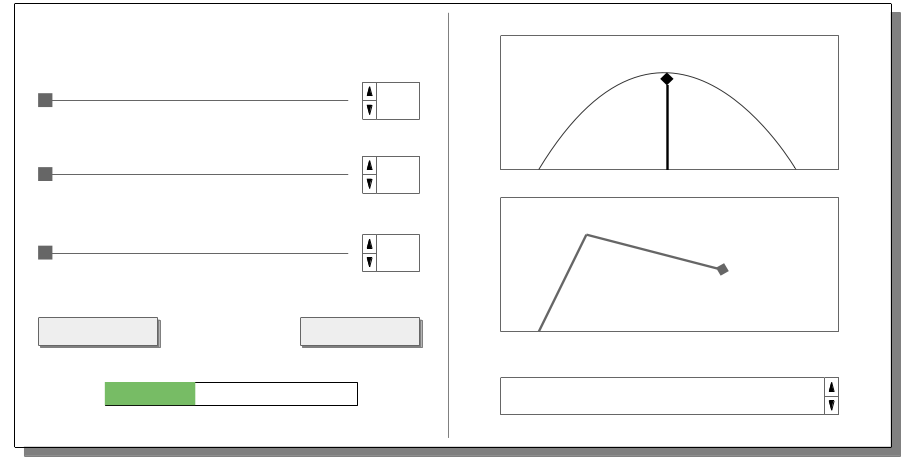
\includegraphics[width=\linewidth]{RS/images/InterfaceSketch-MkII.png}
    \caption{Diseño propuesto para la intefaz gráfica de usuario.}
    \label{fig:ui_design}
\end{figure}

La especificación de los elementos de la interfaz anterior (figura \ref{fig:ui_design}) se hace en mayor profundidad en el punto \ref{sec:ui_reqs} del documento.

\subsection{Memoria}

Por experiencia en proyectos relacionados, se estima que la memoria disponible para 
código y datos, en el microcontrolador seleccionado, ofrecen margen suficiente para este
proyecto. Se detallan a continuación las características a nivel de memoria del
microcontrolador:

\begin{itemize}
    \item 512 KB de memoria \textit{flash}, donde se alberga el programa principal.
    \item 48 KB de memoria \ac{RAM}, donde se alojarán los datos temporales durante la ejecución, teniendo en especial consideración las matrices de las ecuaciones cinemáticas.
\end{itemize}

\subsection{Operaciones}

Los usuarios deberán desempeñar acciones tales que generen los movimientos deseados en el brazo. Estas acciones pueden implicar interactuar con los \textit{widgets} presentes en el panel de control o bien efectuar movimientos con el ratón para que el robot los desempeñe directamente.


\subsection{Funciones del producto}
Las funcionalidades principales del brazo robótico han sido descritas de forma introductoria en apartados anteriores de este documento.

En general, existen dos funcionalidades principales que caracterizan tanto al \pArm{} como al sistema de control del mismo:
\begin{itemize}
    \item La funcionalidad principal del brazo robótico \ac{S2} es la de realizar movimientos dentro de su campo de movimiento y describir trayectorias previamente planificadas o calculadas en el momento. Mediante este movimiento, se pretende transportar objetos de poco peso.
    
    Además, para agilizar el funcionamiento y el procesado de las órdenes, será \ac{S2} el que gestione, compute y realice los movimientos que recibe por parte de \ac{S1}, quedando este último para la interacción con el usuario y la gestión de \ac{S2}.
    
    \item El sistema de control \ac{S1} ofrece la funcionalidad principal de planificar trayectorias y controlar el movimiento del brazo. Este sistema se muestra al usuario mediante una interfaz gráfica, la  cual permite al usuario controlar el movimiento del brazo mediante la modificación de diversos parámetros.
\end{itemize}


\subsection{Características del usuario}
El sistema de control ejecutado en \ac{S1} ofrecerá una interfaz gráfica que permitirá al usuario interactuar con los parámetros del brazo robótico \ac{S2} y, por lo tanto, permitirá al mismo controlar el movimiento del robot así como la establecer la descripción de ciertas trayectorias.

Dado que el objetivo el proyecto es ofrecer un sistema didáctico, amigable y fácil de usar, no se imponen requerimientos específicos sobre el usuario en cuanto a conocimientos técnicos sobre programación, \ac{HW}, electrónica o matemáticos.

El usuario debe estar familiarizado con la interacción y el uso básico de aplicaciones de escritorio para poder interactuar de forma correcta con el sistema de control del brazo.

A pesar de no ser completamente necesario, es recomendable que el usuario esté familiarizado con la estructura física del robot, los movimientos que este puede realizar y los parámetros que se usan para controlar al mismo, ya que de esta forma el control del brazo robótico será más eficaz y seguro.

\subsection{Restricciones}
Dado que actualmente no se presenta ninguna limitación de presupuesto, se busca en el proyecto intentar reducir los costes todo lo posible, para permitir a cualquiera poder acceder a los recursos que se necesitan para desarrollar el proyecto. Por ello, se propone usar el dsPIC33EP512GM604 y montar la placa con los componentes necesarios.

En cualquier caso, como se ha mencionado anteriormente, es necesario que:

\begin{itemize}
    \item Se provea de una interfaz para la comunicación que permita comunicarse con el sistema \ac{S1} de manera simultánea y con alta capacidad.
    \item El sistema ha de consumir la menor energía posible, entrando en el modo de \textit{deep--sleep} cuando fuera posible.
    \item La estructura de \ac{S2} ha de ser imprimible en 3D, permitiendo así replicarlo.
    \item El sistema \ac{S1} ha de poder ejecutar aplicaciones Python según lo propuesto anteriormente, en particular, la versión de este superior a la 3.6. En otro caso, el sistema habrá de poder ejecutar la aplicación diseñada sin problemas e indiferentemente del sistema operativo.
    \item Todo lo realizado en el proyecto ha de ser \ac{OS} y \ac{OH}, permitiendo así que cualquiera pueda acceder y estudiar el proyecto.
\end{itemize}

\subsection{Supuestos y dependencias}
Indiferentemente de la placa que finalmente se use, el sistema ha de tener tres motores: uno para la base, otro para el primer segmento del brazo robótico y el último para el segundo segmento. Además, para controlar el \textit{end--effector} hará falta una conexión con el extremo del brazo que permita, por ejemplo, añadir un pequeño motor que permita la rotación del mismo (ver el manual de desarrollador de UFACTORY para más información).

Para ello, en la tabla \ref{tab:motor_list} se muestran distintas propuestas de motores que podrían ser viables para el proyecto. Intentando cubrir las necesidades, se tienen en cuenta para este proyecto:

\begin{itemize}
    \item Motor paso a paso: dispositivo electromecánico que convierte una serie de pulsos eléctricos en desplazamientos angulares. Esto permite realizar movimientos muy precisos, los cuales pueden variar de $1.8\degree$ hasta $90\degree$.
    \item Servomotor: dispositivos de accionamiento para el control de la velocidad, par motor y posición. En su interior suelen tener un decodificador el cual convierte el giro mecánico en pulsos digitales. Además, suelen disponer de un \textit{driver} el cual permite comandar los distintos controles mencionados al principio.
\end{itemize}

\LTXtable{\linewidth}{RS/content/2/motors_table}

\subsection{Requisitos pospuestos}
En esta sección se describen algunos requisitos del sistema que se postergan a futuras implementaciones o versiones del proyecto.

En el comienzo del proyecto se plantearon algunas funcionalidades y requisitos que, finalmente, se han decidido postergar a futuras implementaciones del proyecto, principalmente debido a su complejidad. En la siguiente lista se presentan las mas relevantes, las cuales representan posibles mejoras futuras del \pArm{}:
\begin{itemize}
    \item Implementación del sistema de control y planificación de trayectorias en el microcontrolador del \pArm{}, de esta forma se busca centralizar el computo en \ac{S2}.
    \item Implementación de un sistema de descripción de trayectorias mediante imitación de movimientos realizados por el usuario, es decir, el usuario podría mover físicamente el \pArm{} y memorizaría dicha trayectoria para posteriormente describirla.
    \item Construcción e implementación de diversos tipos de \textit{end--effector} para el \pArm{}, los cuales le dotarían de nuevas funcionalidades en cuanto a manejar objetos.
    \item Implementación de las estructura física del \pArm{} utilizando materiales metálicos para mejorar su resistencia y estabilidad. Junto con esta mejora, se podrían utilizar nuevos rotores para dotar al \pArm{} de una mayor capacidad de carga.
\end{itemize}

  

\newpage

\section{Requisitos específicos}
\label{Requisitos específicos}

%\subsection{User Interfaces}

\subsection{Requisitos de la interfaz externa}
\subsubsection{Interfaz con el usuario}
\label{sec:ui_reqs}
\ac{S1} dispondrá de una interfaz de usuario que deberá seguir el modelo propuesto en la figura \ref{fig:ui_design}. Dicha interfaz habrá de contar con los siguientes elementos:
\begin{itemize}
    \item Distintos controladores gráficos que permitan establecer la posición final del \textit{end--effector} bien mediante coordenadas articulares o bien mediante coordenadas angulares.
    \item Un actuador para poder escoger entre las alternativas mencionadas en el punto anterior.
    \item Un actuador para confirmar que se quiere mandar el movimiento al brazo robótico.
    \item Un actuador para detener un movimiento en ejecución del brazo.
\end{itemize}

Teniendo en cuenta el diseño propuesto en la figura \ref{fig:ui_design}, los componentes anteriores estarían
representados por:

\begin{itemize}
    \item Tres \textit{slider}s los cuales establecerán los valores para los ángulos 
    $\left\{\theta_1, \theta_2, \theta_3\right\}$, si se está trabajando en el modo de coordenadas
    angulares; o los valores de los puntos $\left\{x, y, z\right\}$, si se está trabajando en el modo
    de coordenadas cartesianas.
    \item Un botón desplegable con múltiples opciones que permitiría escoger entre los dos modos
    mencionados en el punto anterior.
    \item Un botón que permita confirmar los cambios en las coordenadas/ángulos antes de enviar
    definitivamente el movimiento al robot.
    \item Una barra de progreso la cual permite conocer una estimación de cuánto lleva el robot hecho
    del movimiento final previsto.
    \item Dos pequeñas ventanas que informan sobre la posición del brazo final una vez se han
    cambiado los valores de las coordenadas/ángulos. Dichas ventanas muestra una vista cenital del
    brazo, que indica cómo se mueve en el eje $Y$, y una vista de perfil del mismo, que indica cómo
    se mueve en el eje $XZ$.
    \item Una pequeña ventana que muestra \textit{logs} relevantes respecto a la situación tanto
    de \ac{S1} como de \ac{S2}.
\end{itemize}
\subsection{Interfaz \textit{hardware}}
\ac{S2} esta formado por el brazo robótico \pArm{} y el microcontrolador que computa las instrucciones recibidas desde \ac{S1}. Mediante dicho microcontrolador, \ac{S2} interactúa directamente con el \ac{HW}. El microcontrolador realiza las labores de comunicación con \ac{S1}, así como las labores de recepción y procesamiento de las instrucciones que controlan el movimiento del \pArm{}.

Tras la recepción y procesamiento de las diferentes secuencias de bits, las cuales son instrucciones, el microcontrolador genera señales de salida mediante sus pines, las cuales controlan el movimiento de cada uno de los motores, así como del \textit{end--effector}. Cabe destacar que, en el caso de utilizar motores que proporcionen información sobre su posición angular actual, el microcontrolador debe recibir dicha señal y procesarla, enviando dicha información a \ac{S1}.

Dependiendo del tipo de motores que se utilicen finalmente, el microcontrolador debe ser capaz de generar señales analógicas \ac{PWM}, así como señales digitales de control.





\subsubsection{Interfaz de comunicaciones}
Las comunicaciones que se realicen entre \ac{S1} y \ac{S2} están planteadas para utilizar \ac{UART} como método de comunicación. Además, se mencionó como futura implementación poder hacer las comunicaciones entre ambos sistemas utilizando protocolos de red inalámbricos.

No se restringe la velocidad de transmisión (\textit{baud--rate}), ya que se asume que \ac{S1} tendrá la posibilidad de adaptar su velocidad. Se escoge el \ac{USB} como método para intercambiar la información debido a:

\begin{itemize}
    \item Universalidad: los dispositivos cuentan con al menos una conexión \ac{USB}.
    \item Energía: el \ac{USB} provee $5~V$ al circuito que se conecta en el otro extremo. Además, la versión 2.0 del estándar, que es lo generalizado en microcontroladores, puede proveer hasta $500~mA$ al componente conectado.
    \item Simplicidad: no es necesario entender cómo se conectan los cables sino directamente conectar los extremos.
\end{itemize}

Para un correcto funcionamiento, la comunicación ha de ser bidireccional, en particular \textit{full duplex}. De esta forma, se podrán recibir y enviar datos simultáneamente, pudiendo así conocer el estado del brazo robótico y actuar en consecuencia en caso de que se encuentre algún tipo de error o problema. Al utilizar el \ac{USB} como método de comunicación este problema está subsanado, ya que va implícito en la definición del estándar.

\subsection{Casos de uso}
\begin{figure}[H]
    \centering
    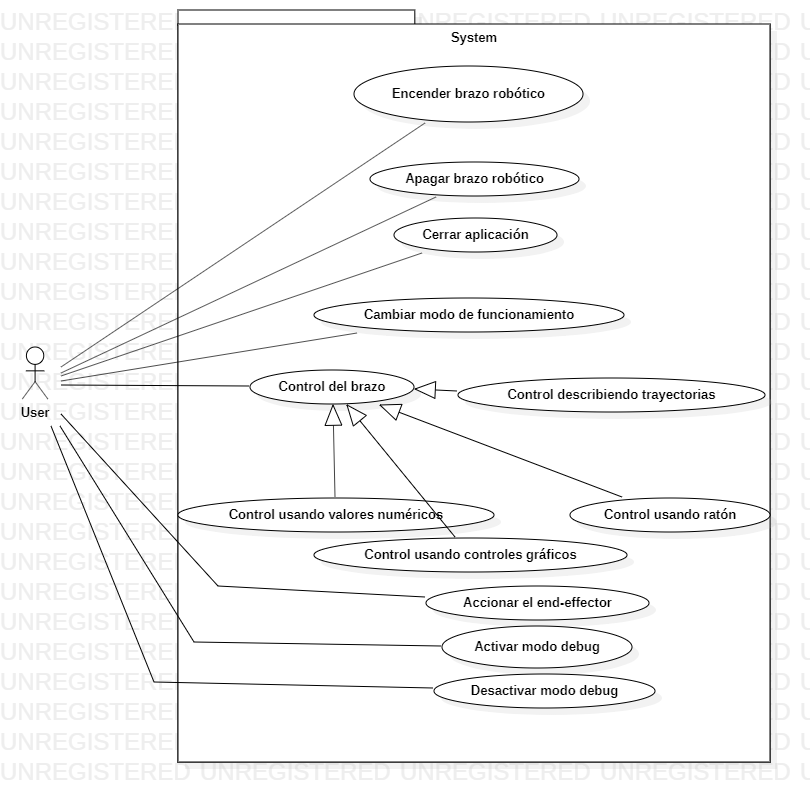
\includegraphics[width=.7\textwidth]{RS/images/UseCaseDiagram1.png}
    \caption{Diagrama de casos de uso}
    \label{fig:diagrama_casos_uso}
\end{figure}


\begin{table}[H]
    \centering
    \begin{tabularx}{\textwidth}{|c|c|X|}
        \cline{1-3}
        \texttt{0001}                              & \multicolumn{2}{c|}{Encender brazo robótico (\ac{S2})}                                                                                                                      \\ \cline{1-3}
        \textbf{Descripción}                       & \multicolumn{2}{m{13cm}|}{El usuario deberá se capaz de encender el sistema del brazo robótico de manera independiente de la aplicación de control.}
        \\ \cline{1-3}
        \multirow{4}{*}{\textbf{Secuencia Normal}} & \textbf{Paso} & \textbf{Acción}
        \\ \cline{2-3}                    &   1  & El usuario interactúa con el sistema para encenderlo.
        \\ \cline{2-3}                    &   2  & El sistema comprueba que los motores están correctamente conectados.
        \\ \cline{2-3}                    &   3  & Si las comprobaciones son satisfactorias, el sistema continúa con su normal ejecución.
        \\ \cline{1-3}
        \multirow{2}{*}{\textbf{Excepciones}}      & \textbf{Paso}                                                                                                                                        & \textbf{Acción}
        \\ \cline{2-3}                    &   3  & Si las comprobaciones no son satisfactorias el sistema activará un indicador luminoso y se informará del error a \ac{S1}, si está conectado.
        \\ \cline{1-3}
        \textbf{Importancia}                       & \multicolumn{2}{c|}{1}                                                                                                                                                 \\ \cline{1-3}
        \textbf{Comentarios}                       & \multicolumn{2}{c|}{Sin comentarios}                                                                                                                                   \\ \cline{1-3}
    \end{tabularx}
    \caption{Caso de uso \texttt{0001} - Encender brazo robótico (\ac{S2}).}
    \label{tab:CU0001}
    \label{tab:caso_de_uso_encender_brazo_robotico}
\end{table}

\begin{table}[H]
    \centering
    \begin{tabularx}{\textwidth}{|c|c|X|}
        \cline{1-3}
        \texttt{0002}                              & \multicolumn{2}{c|}{Apagar brazo robótico(\ac{S2})}                    \\ \cline{1-3}
        \textbf{Descripción}                       & \multicolumn{2}{m{13cm}|}{El usuario deberá ser capaz de apagar el brazo robótico desconectando la corriente del mismo.}
        \\ \cline{1-3}
        \multirow{4}{*}{\textbf{Secuencia Normal}} & \textbf{Paso}  & \textbf{Acción}
        \\ \cline{2-3}                             &   1            & El usuario interactúa con el sistema para apagarlo.
        \\ \cline{2-3}                             &   2            & El sistema se apaga.
        \\ \cline{1-3}
        \multirow{2}{*}{\textbf{Excepciones}}      & \textbf{Paso}                                                                                                                                        & \textbf{Acción}
        \\ \cline{2-3}                    &     & No existen
        \\ \cline{1-3}
        \textbf{Importancia}                       & \multicolumn{2}{c|}{1}                                                                                                                                                 \\ \cline{1-3}
        \textbf{Comentarios}                       & \multicolumn{2}{c|}{Sin comentarios}                                                                                                                                   \\ \cline{1-3}
    \end{tabularx}
    \caption{Caso de uso \texttt{0002} - Apagar brazo robótico (\ac{S2}).}
    \label{tab:CU0002}
    \label{tab:caso_de_uso_apagar_brazo_robotico}
\end{table}

\begin{table}[H]
    \centering
    \begin{tabularx}{\textwidth}{|c|c|X|}
        \cline{1-3}
        \texttt{0003}        & \multicolumn{2}{c|}{Cerrar aplicación}                                                       
        \\ \cline{1-3}
        \textbf{Descripción} & \multicolumn{2}{m{13cm}|}{El usuario deberá ser capaz de cerrar la aplicación de control de manera independiente al brazo robótico.}
        \\ \cline{1-3}
        \multirow{4}{*}{\textbf{Secuencia Normal}} & \textbf{Paso} & \textbf{Acción}
        \\ \cline{2-3}                    &   1  & El usuario interactúa con la aplicación para cerrarla
        \\ \cline{2-3}                    &   2  & Se comprueba que la  aplicación se puede cerrar de manera segura. Esto implica asegurar que no hay ninguna comunicación en proceso antes de cerrar la apliación
        \\ \cline{2-3}                    &   3  & Se realiza el cierre de la aplicación.
        \\ \cline{1-3}
        \multirow{2}{*}{\textbf{Excepciones}} & \textbf{Paso} & \textbf{Acción}
        \\ \cline{2-3}                        &  2  & La aplicación no se puede cerrar de manera segura.
        \\ \cline{2-3}                        & 2.1 & Se impide el cierre
        \\ \cline{1-3}
        \textbf{Importancia}                 & \multicolumn{2}{c|}{1}           
        \\ \cline{1-3}
        \textbf{Comentarios}                 & \multicolumn{2}{c|}{Sin comentarios}
        \\ \cline{1-3}
    \end{tabularx}
    \caption{Caso de uso \texttt{0003} - Cerrar aplicación.}
    \label{tab:CU0003}
    \label{tab:caso_de_uso_cerrar_aplicación}
\end{table}


\begin{table}[H]
    \centering
    \begin{tabularx}{\textwidth}{|c|c|X|}
        \cline{1-3}
        \texttt{0004}                              & \multicolumn{2}{c|}{Cambiar modo de funcionamiento (\ac{S1})}                                                                                                                      \\ \cline{1-3}
        \textbf{Descripción}                       & \multicolumn{2}{m{13cm}|}{El usuario deberá ser capaz de seleccionar el modo de control del brazo robótico, pudiendo escoger entre control mediante ratón o control mediante parámetros. }
        \\ \cline{1-3}
        \multirow{4}{*}{\textbf{Secuencia Normal}} & \textbf{Paso}                                                                                                                                        & \textbf{Acción}
        \\ \cline{2-3}                    &   1  & El usuario interactúa con la aplicación y selecciona el modo de control del robot.
        \\ \cline{2-3}                    &   2  & El sistema cambia entre modo de control mediante ratón o modo de control mediante parámetros.
        \\ \cline{1-3}
        \multirow{2}{*}{\textbf{Excepciones}}      & \textbf{Paso}                                                                                                                                        & \textbf{Acción}
        \\ \cline{2-3}                    &     &  No existen
        \\ \cline{1-3}
        \textbf{Importancia}                       & \multicolumn{2}{c|}{1}                                                                                                                                                 \\ \cline{1-3}
        \textbf{Comentarios}                       & \multicolumn{2}{c|}{Sin comentarios}                                                                                                                                   \\ \cline{1-3}
    \end{tabularx}
    \caption{Caso de uso \texttt{0004} - Cambiar modo de funcionamiento.}
    \label{tab:CU0004}
    \label{tab:caso_de_uso_cambiar_modo_de_funcionamiento}
\end{table}


\begin{table}[H]
    \centering
    \begin{tabularx}{\textwidth}{|c|c|X|}
        \cline{1-3}
        \texttt{0005}                              & \multicolumn{2}{c|}{Control usando valores numéricos (\ac{S1})}                                                                                                                      \\ \cline{1-3}
        \textbf{Descripción}                       & \multicolumn{2}{m{13cm}|}{El usuario deberá ser capaz de cambiar el valor numérico de cada uno de los parámetros de control del brazo robótico}
        \\ \cline{1-3}
        \multirow{4}{*}{\textbf{Secuencia Normal}} & \textbf{Paso}                                                                                                                                        & \textbf{Acción}
        \\ \cline{2-3}                    &   1  & El usuario interactúa con la aplicación y cambia el valor de los parámetros de control usando el teclado.
        \\ \cline{2-3}                    &   2  & Se comprueba si el valor es correcto y se confirma el cambio del valor numérico.
        \\ \cline{1-3}
        \multirow{2}{*}{\textbf{Excepciones}} & \textbf{Paso}  & \textbf{Acción}
        \\ \cline{2-3}                        &   2  & El valor introducido por el usuario no es correcto y por lo tanto no puede llevarse a la práctica.
        \\ \cline{2-3} 
                                              &  2.1 & Se elimina el valor y se notifica al usuario sobre el error y se le pide que introduzca de nuevo el valor.
        \\ \cline{1-3}
        \textbf{Importancia}                       & \multicolumn{2}{c|}{1}                                                                                                                                                 \\ \cline{1-3}
        \textbf{Comentarios}                       & \multicolumn{2}{c|}{Sin comentarios}                                                                                                                                   \\ \cline{1-3}
    \end{tabularx}
    \caption{Caso de uso \texttt{0005} - Control usando valores numéricos (\ac{S1}).}
    \label{tab:CU0005}
    \label{tab:caso_de_uso_control_usando_valores_numericos}
\end{table}

\begin{table}[H]
    \centering
    \begin{tabularx}{\textwidth}{|c|c|X|}
        \cline{1-3}
        \texttt{0006}        & \multicolumn{2}{c|}{Control describiendo trayectorias}                                      
        \\ \cline{1-3}
        \textbf{Descripción} & \multicolumn{2}{m{13cm}|}{Se permitirá al usuario escoger una trayectoria predefinida que el brazo robótico deberá realizar.}
        \\ \cline{1-3}
        \multirow{4}{*}{\textbf{Secuencia Normal}} & \textbf{Paso} & \textbf{Acción}
        \\ \cline{2-3}                    &   1  & El usuario selecciona una trayectoria a realizar.
        \\ \cline{2-3}                    &   2  & Se realiza dicha trayectoria
        \\ \cline{1-3}
        \multirow{2}{*}{\textbf{Excepciones}} & \textbf{Paso} & \textbf{Acción}
        \\ \cline{2-3}                    &      &  No existen
        \\ \cline{1-3}
        \textbf{Importancia}                 & \multicolumn{2}{c|}{1}           
        \\ \cline{1-3}
        \textbf{Comentarios}                 & \multicolumn{2}{m{13cm}|}{\textbf{Esta característica no se implementa ya que se posterga para una futura versión.}}
        \\ \cline{1-3}
    \end{tabularx}
    \caption{Caso de uso \texttt{0006} - Control describiendo trayectorias.}
    \label{tab:CU0006}
    \label{tab:caso_de_uso_control_describiendo_trayectorias}
\end{table}

\begin{table}[H]
    \centering
    \begin{tabularx}{\textwidth}{|c|c|X|}
        \cline{1-3}
        \texttt{0007}        & \multicolumn{2}{c|}{Control usando controles gráficos}                                      
        \\ \cline{1-3}
        \textbf{Descripción} & \multicolumn{2}{m{13cm}|}{La interfaz gráfica de la aplicación debe ofrecer control sobre los parámetros del brazo robótico mediante \textit{sliders}.}
        \\ \cline{1-3}
        \multirow{4}{*}{\textbf{Secuencia Normal}} & \textbf{Paso} & \textbf{Acción}
        \\ \cline{2-3}                    &   1  & El usuario interactúa con la aplicación y mueve los \textit{sliders} para variar los parámetros del brazo robótico.
        \\ \cline{2-3}                    &   2  & Se verifica si se puede realizar dicho movimiento y se ejecuta el cambio en los parámetros.
        \\ \cline{1-3}
        \multirow{2}{*}{\textbf{Excepciones}} & \textbf{Paso} & \textbf{Acción}
        \\ \cline{2-3}                    &   2   &  La posición no es alcanzable o no se puede llevar a la práctica.
        \\ \cline{2-3}                    &  2.1  &  Se notifica el error.
        \\ \cline{1-3}
        \textbf{Importancia}                 & \multicolumn{2}{c|}{1}           
        \\ \cline{1-3}
        \textbf{Comentarios}                 & \multicolumn{2}{c|}{Sin comentarios}
        \\ \cline{1-3}
    \end{tabularx}
    \caption{Caso de uso \texttt{0007} - Control usando controles gráficos.}
    \label{tab:CU0007}
    \label{tab:caso_de_uso_control_usando_controles_graficos}
\end{table}

\begin{table}[H]
    \centering
    \begin{tabularx}{\textwidth}{|c|c|X|}
        \cline{1-3}
        \texttt{0008}        & \multicolumn{2}{c|}{Control usando ratón}                                      
        \\ \cline{1-3}
        \textbf{Descripción} & \multicolumn{2}{m{13cm}|}{Se permitirá al usuario controlar el brazo robótico de manera directa con el movimiento del ratón}
        \\ \cline{1-3}
        \multirow{4}{*}{\textbf{Secuencia Normal}} & \textbf{Paso} & \textbf{Acción}
        \\ \cline{2-3}                    &   1  & El usuario mueve el ratón realizando movimientos libres.
        \\ \cline{2-3}                    &   2  & Se comprueba que el movimiento no se sale de los margenes permitidos
        \\ \cline{2-3}                    &   3  & Se realiza el movimiento
        \\ \cline{1-3}
        \multirow{2}{*}{\textbf{Excepciones}} & \textbf{Paso} & \textbf{Acción}
        \\ \cline{2-3}                    &   2   &  Si los movimientos se salen de los margenes permitidos no se realizan.
        \\ \cline{1-3}
        \textbf{Importancia}                 & \multicolumn{2}{c|}{1}           
        \\ \cline{1-3}
        \textbf{Comentarios}                 & \multicolumn{2}{m{13cm}|}{\textbf{Esta característica no se implementa ya que se posterga para una futura versión.}}
        \\ \cline{1-3}
    \end{tabularx}
    \caption{Caso de uso \texttt{0008} - Control usando ratón.}
    \label{tab:CU0008}
    \label{tab:caso_de_uso_control_usando_ratón}
\end{table}

\begin{table}[H]
    \centering
    \begin{tabularx}{\textwidth}{|c|c|X|}
        \cline{1-3}
        \texttt{0009}        & \multicolumn{2}{c|}{Accionar el \textit{end--effector}}                                      
        \\ \cline{1-3}
        \textbf{Descripción} & \multicolumn{2}{m{13cm}|}{Se permite al usuario abrir y cerrar la pinza}
        \\ \cline{1-3}
        \multirow{4}{*}{\textbf{Secuencia Normal}} & \textbf{Paso} & \textbf{Acción}
        \\ \cline{2-3}                    &   1  & El usuario interactúa con la aplicación para abrir y cerrar el \textit{end--effector}
        \\ \cline{2-3}                    &   2  & Se cambia el estado del \textit{end--effector} según sea necesario. 
        \\ \cline{1-3}
        \multirow{2}{*}{\textbf{Excepciones}} & \textbf{Paso} & \textbf{Acción}
        \\ \cline{2-3}                    &      &  No existe
        \\ \cline{1-3}
        \textbf{Importancia}                 & \multicolumn{2}{c|}{1}           
        \\ \cline{1-3}
        \textbf{Comentarios}                 & \multicolumn{2}{m{13cm}|}{\textbf{Esta característica no se implementa ya que se posterga para una futura versión.}}
        \\ \cline{1-3}
    \end{tabularx}
    \caption{Caso de uso \texttt{0009} - Accionar el \textit{end--effector}.}
    \label{tab:CU0009}
    \label{tab:caso_de_uso_accionar_end_effector}
\end{table}

\begin{table}[H]
    \centering
    \begin{tabularx}{\textwidth}{|c|c|X|}
        \cline{1-3}
        \texttt{0010}        & \multicolumn{2}{c|}{Activar modo \textit{debug}}                                      
        \\ \cline{1-3}
        \textbf{Descripción} & \multicolumn{2}{m{13cm}|}{Se permite al usuario activar un modo tal que se pueda mandar al \ac{S2} el código de control del brazo robótico}
        \\ \cline{1-3}
        \multirow{4}{*}{\textbf{Secuencia Normal}} & \textbf{Paso} & \textbf{Acción}
        \\ \cline{2-3}                    &   1  & El usuario interactúa con S2 para ponerlo en modo debug.
        \\ \cline{2-3}                    &   2  & El sistema comprueba que el cambio de modo se puede hacer de manera segura. Es decir, no hay una comuniación en proceso antes de realizar el cambio de modo.
        \\ \cline{2-3}                    &   3  & El sistema cambia de modo.
        \\ \cline{1-3}
        \multirow{2}{*}{\textbf{Excepciones}} & \textbf{Paso} & \textbf{Acción}
        \\ \cline{2-3}                    &   2  & El sistema detecta que el cambio de modo no se puede hacer de manera segura e impide que este se realice. Se informará del error a \ac{S1}, si está conectado.
        \\ \cline{1-3}
        \textbf{Importancia}                 & \multicolumn{2}{c|}{1}           
        \\ \cline{1-3}
        \textbf{Comentarios}                 & \multicolumn{2}{m{13cm}|}{\textbf{Esta característica no se implementa ya que se posterga para una futura versión.}}
        \\ \cline{1-3}
    \end{tabularx}
    \caption{Caso de uso \texttt{0010} - Activar el modo \textit{debug}.}
    \label{tab:CU0010}
    \label{tab:caso_de_uso_activar_modo_debug}
\end{table}

\begin{table}[H]
    \centering
    \begin{tabularx}{\textwidth}{|c|c|X|}
        \cline{1-3}
        \texttt{0011}        & \multicolumn{2}{c|}{Desactivar modo \textit{debug}}                                      
        \\ \cline{1-3}
        \textbf{Descripción} & \multicolumn{2}{m{13cm}|}{Se permite al usuario desactivar el modo debug tal que sea posible emplear el sistema de manera normal}
        \\ \cline{1-3}
        \multirow{4}{*}{\textbf{Secuencia Normal}} & \textbf{Paso} & \textbf{Acción}
        \\ \cline{2-3}                    &   1  & El usuario interactúa con \ac{S2} para desactivar el modo debug.
        \\ \cline{2-3}                    &   2  & El sistema comprueba que el cambio de modo se puede hacer de manera segura.
        \\ \cline{2-3}                    &   3  & El sistema cambia de modo.
        \\ \cline{1-3}
        \multirow{2}{*}{\textbf{Excepciones}} & \textbf{Paso} & \textbf{Acción}
        \\ \cline{2-3}                    &   2  & El sistema detecta que el cambio de modo no se puede hacer de manera segura e impide que este se realice. Se informara del error a \ac{S1}, si esta conectado.
        \\ \cline{1-3}
        \textbf{Importancia}                 & \multicolumn{2}{c|}{1}           
        \\ \cline{1-3}
        \textbf{Comentarios}                 & \multicolumn{2}{m{13cm}|}{\textbf{Esta característica no se implementa ya que se posterga para una futura versión.}}
        \\ \cline{1-3}
    \end{tabularx}
    \caption{Caso de uso \texttt{0011} - Desactivar el modo \textit{debug}.}
    \label{tab:CU0011}
    \label{tab:caso_de_uso_desactivar_modo_debug}
\end{table}

\subsection{Requisitos funcionales}
\subsubsection{Permitir generar movimientos}
\subsubsection*{ -- Mediante el ángulo de cada uno de los motores}

El sistema \ac{S2} cuenta con tres motores los cuales se encargan del movimiento de cada una de las partes del
brazo. Se permitirá establecer individualmente cada ángulo $\left\{\theta_0, \theta_2, \theta_3\right\}$ 
y mover así el brazo a una posición final $\left\{x', y', z'\right\}$.

Este movimiento, siguiendo la maqueta definida en la figura \ref{fig:ui_design}, se realizará interactuando
con \textit{sliders}.

\subsubsection*{ -- Mediante las coordenadas cartesianas del punto final}
Se permitirá también el movimiento a un punto $\left\{x, y, z\right\}$ directamente, para lo que se obtendrán
los ángulos $\left\{\theta_0, \theta_2, \theta_3\right\}$ que permiten alcanzar dicha posición.

Al igual que en el caso anterior, se podrá definir cada punto independientemente.

Este movimiento, siguiendo la maqueta definida en la figura \ref{fig:ui_design}, se realizará interactuando
con \textit{sliders}.

\subsubsection*{ -- Selección del modo de funcionamiento del brazo}
Dado que, como se ha mencionado en los puntos anteriores, hay dos maneras de hacer que el brazo se pueda
mover, habrá de existir algún tipo de actuador en la interfaz de usuario que permita escoger entre dichos modos.

Esta acción, siguiendo la maqueta definida en la figura \ref{fig:ui_design}, se realizará interactuando con
un botón.

\subsubsection*{ -- Ejecución en un momento determinado}
La interacción con los elementos comentados anteriormente no será efectiva hasta que el usuario indique que
quiere que se realicen, permitiendo así confirmar que los datos introducidos son los correctos.

Esta acción, siguiendo la maqueta definida en la figura \ref{fig:ui_design}, se realizará interactuando con
un botón.

\subsubsection*{ -- Demostración del punto final del brazo}
La interacción con los actuadores definidos anteriormente se verá reflejada en unas pequeñas ventanas
que muestran cómo debería encontrarse el brazo tras realizar los movimientos indicados.

Esta demostración, siguiendo la maqueta definida en la figura \ref{fig:ui_design}, se mostrará mediante
unos dibujos esquemáticos que representan el brazo visto de perfil y desde una vista cenital.

\subsubsection*{ -- Otros requisitos}
Se han considerado operaciones más avanzadas para el control del brazo (como trazar trayectorias o
un control mediante el ratón en un plano 2D) las cuales no se reflejan en este documento ya que se
ha postergado su desarrollo e implementación a una futura versión del sistema.

% \subsubsection{Requisitos \textit{software}}
% \subsection*{\ac{S1}}
\subsubsection{Mostrar pantalla de control}
\begin{itemize}
    \item ID: 1
    \item Prioridad: 3.
    \item Descripción: se muestra una pantalla donde serán situados los \textit{sliders}.
    \item Entradas: ninguna.
    \item Salidas: ninguna.
    \item Errores: no se espera ningún error.
\end{itemize}

\subsubsection{Mostrar pantalla informativa}
\begin{itemize}
    \item ID: 2
    \item Prioridad: 2
    \item Descripción: se mostrarán distintos datos informativos sobre el estado del sistema \ac{S2}, en caso de que este se haya conectado correctamente.
    \item Entradas: los datos recibidos por el sistema \ac{S2}, si estuviera conectado.
    \item Salidas: los datos recibidos debidamente interpretados por el sistema.
    \item Errores: se mostrará un aviso en caso de que el sistema \ac{S2} no se detecte o presente algún problema.
\end{itemize}

\subsubsection{Mostrar botones de edición de pantalla}
\begin{itemize}
    \item ID: 3
    \item Prioridad: 2
    \item Descripción: se muestran \textit{widgets} de tipo botones clicables de minimizar, maximizar y cerrar pantalla.
    \item Entradas: ninguna.
    \item Salidas: ninguna.
    \item Errores: en caso de que algún proceso pudiera quedar bloqueado, los \textit{widgets} permitirían el cierre inmediato de la aplicación.
\end{itemize}

\subsubsection{Interactuar con botones de edición de pantalla}
\begin{itemize}
    \item ID: 4
    \item Prioridad: 3.
    \item Descripción: se permite interactuar con los botones que aparecen en la \ac{GUI} para controlar la pantalla \ac{S2}.
    \item Entradas: interacción del usuario con los botones de edición de pantalla.
    \item Salidas: cambios lógicos tales que se realicen los cometidos de cada botón.
    \item Errores: no se espera ningún error.
\end{itemize}

\subsubsection{Mostrar \textit{sliders}}
\begin{itemize}
    \item ID: 5
    \item Prioridad: 3.
    \item Descripción: se muestra por pantalla una serie de \textit{widgets} de tipo \textit{sliders}.  
    \item Entradas: coordenadas angulares $\left(\theta_1, \theta_2, \theta_3\right)$ y coordenadas cartesianas $\left(X,Y,Z\right)$.
    \item Salidas: mostrar por pantalla de manera gráfica el valor de las variables.
    \item Errores: no se espera ningún error.
\end{itemize}

\subsubsection{Editar la posición de los \textit{sliders}}
\begin{itemize}
    \item ID: 6
    \item Prioridad: 3.
    \item Descripción: se permite al usuario interactuar de manera directa e independiente con cada uno de los motores del brazo robótico, así como con las componentes de la posición cartesiana del \textit{end--effector}. Este requisito permite al usuario tener una mayor precisión en cuanto a la posición que desea obtener para el brazo robótico.
    \item Entradas: variación por parte del usuario de la posición de los \textit{sliders}.
    \item Salidas: modificar el valor numérico de las variables.
    \item Errores: no se espera ningún error.
\end{itemize}

\subsubsection{Mostrar botón cambio de modo de funcionamiento del \ac{S1}}
\begin{itemize}
    \item ID: 7
    \item Prioridad: 3.
    \item Descripción: se muestra por pantalla un \textit{widget} de tipo botón clicable que permite cambiar el modo de funcionamiento. 
    \item Entradas: al hacer clic se permite el cambio de modo.
    \item Salidas: mostrar el nuevo modo de funcionamiento.
    \item Errores: no se espera ningún error.
\end{itemize}

\subsubsection{Interactuar con botón de cambio de modo de funcionamiento del \ac{S1}}
\begin{itemize}
    \item ID: 8
    \item Descripción: se permite al usuario interactuar con el botón para cambiar el modo de funcionamiento.
    \item Entradas: interacción del usuario con el botón.
    \item Salidas: modificación del modo de funcionamiento.
    \item Errores: no se espera ningún error.
\end{itemize}

\subsubsection{Mostrar variables}
\begin{itemize}
    \item ID: 9
    \item Prioridad: 2.
    \item Descripción: se muestran por pantalla las variables que definen las posiciones cartesianas del \textit{end--effector} y las angulares de los motores.
    \item Entradas: valores numéricos de las variables.
    \item Salidas: mostrar por pantalla dichos valores.
    \item Errores: no se espera ningún error.
\end{itemize}

\subsubsection{Mostrar botón de control del \textit{end--effector}}
\begin{itemize}
    \item ID: 10
    \item Prioridad: 2.
    \item Descripción: se muestra por pantalla un \textit{widget} de tipo botón clicable que permite cambiar el estado del \textit{end--effector}.
    \item Entradas: estado del \textit{end--effector}
    \item Salidas: mostrar el estado de \textit{end--effector}.
    \item Errores: no se espera ningún error.
\end{itemize}

\subsubsection{Interactuar con botón de control del \textit{end--effector}}
\begin{itemize}
    \item ID: 11
    \item Prioridad: 2.
    \item Descripción: se permite al usuario interactuar con el el botón para cambiar el estado de la pinza
    \item Entradas: interacción con el botón por parte del usuario.
    \item Salidas: modificar el estado del \textit{end--effector}.
    \item Errores: no se espera ningún error.
\end{itemize}

\subsubsection{Editar variables}
\begin{itemize}
    \item ID: 12
    \item Prioridad: 3.
    \item Descripción: se permite al usuario editar las variables numéricas de manera directa interactuando con el campo y escribiendo los valores numéricos deseados.
    \item Entradas: cambio por parte del usuario del valor numérico mostrado.
    \item Salidas: modificar el valor numérico de la variable.
    \item Errores: no se espera ningún error.
\end{itemize}

\subsubsection{Comprobar variables}
\begin{itemize}
    \item ID: 13
    \item Prioridad: 3.
    \item Descripción: El sistema, al detectar cambios en alguna de las coordenadas, ya sean cartesianas o angulas se encarga de verificar que dichas coordenadas están en el rango de trabajo del robot. De no ser así se impide el movimiento del brazo para prevenir daños en su estructura o en los motores.
    \item Entradas: valor de las coordenadas angulares y cartesianas deseadas.
    \item Salidas: validación de dichas coordenadas.
    \item Errores: si alguno de los valores introducidos no es válido, se notificará al usuario de dicho error y se evitará que el \ac{S2} realice dichos movimientos.
\end{itemize}

\subsubsection{Comunicación con el sistema \ac{S2}}
\begin{itemize}
    \item ID: 14
    \item Prioridad: 1.
    \item Descripción: utilizando un lenguaje binario, se comunicarán las secuencias de órdenes desde el sistema \ac{S1} al sistema \ac{S2}.
    \item Entradas: secuencia de movimientos representada como movimientos en puntos cartesianos o como rotaciones de las articulaciones.
    \item Salidas: secuencia binaria que especifica, en el sistema \ac{S2}, los movimientos que se han de realizar.
    \item Errores: como se han comprobado los elementos con anterioridad, no se esperan errores.
\end{itemize}

\subsubsection{Cálculo de coordenadas articulares}
\begin{itemize}
    \item ID: 15
    \item Prioridad: 1.
    \item Descripción: dadas unas coordenadas en forma cartesiana, el sistema \ac{S1} debe poder calcular las coordenadas articulares de cada una de las articulaciones del robot.
    \item Entradas: conjunto de tres puntos cartesianos $(X,Y,Z)$.
    \item Salidas: conjunto de tres puntos articulares $(\theta_1, \theta_2, \theta_3)$.
    \item Errores: dada la configuración geométrica del robot, no se esperan errores.
\end{itemize}

\subsubsection{Cálculo de coordenadas cartesianas}
\begin{itemize}
    \item ID: 16
    \item Prioridad: 1.
    \item Descripción: dadas unas coordenadas articulares, el sistema \ac{S1} debe poder obtener las coordenadas cartesianas en las que se encuentra en \textit{end--effector}.
    \item Entradas: conjunto de tres puntos articulares $(\theta_1, \theta_2, \theta_3)$.
    \item Salidas: conjunto de tres puntos cartesianos $(X,Y,Z)$.
    \item Errores: no se esperan errores.
\end{itemize}

\subsubsection{Interpretación de los datos}
\begin{itemize}
    \item ID: 17
    \item Prioridad: 1.
    \item Descripción: el sistema \ac{S1} debe de poder entender e interpretar los datos recibidos desde \ac{S2}.
    \item Entradas: cadena binaria con información provista por \ac{S2}.
    \item Salidas: mostrar, utilizando la interfaz de usuario, la información pertinente.
    \item Errores: no se esperan errores.
\end{itemize}

\subsubsection{Protocolo de intercambio de información}
\begin{itemize}
    \item ID: 18
    \item Prioridad: 1.
    \item Descripción: debe existir un protocolo de intercambio de información que defina la longitud, significado y estructura del las instrucciones o secuencias de bits que se transmiten mediante \textit{UART}.
    \item Entradas: Ninguna.
    \item Salidas: Ninguna.
\end{itemize}    

\subsubsection{Encendido del sistema}
\begin{itemize}
    \item ID: 19
    \item Prioridad: 0.
    \item Descripción: el \ac{S1}, al encenderse, debe comprobar si está conectado el \ac{S2} e inicializar aquellos recursos que serán necesarios.
    \item Entradas: ninguna.
    \item Salidas: ninguna.
    \item Errores: se esperan errores si hubiera algún tipo de corrupción de datos en los ficheros del programa o en los contenedores de datos.
\end{itemize}

\subsubsection{Apagado del sistema}
\begin{itemize}
    \item ID: 20
    \item Prioridad: 1.
    \item Descripción: cuando el usuario cierra la interfaz, el sistema \ac{S1} debe desconectarse del todo y cesar cualquier comunicación que pudiera existir con \ac{S2}. Además, deberá eliminar cualquier tipo de dato residual resultante.
    \item Entradas: el usuario cierra la aplicación.
    \item Salidas: ninguna.
    \item Errores: se esperan errores si no fuese posible cesar la comunicación debido a alguna política del sistema operativo. Se notificará al usuario al respecto.
\end{itemize}

\subsection*{\ac{S2}} 
\subsubsection{Encendido del sistema}
\begin{itemize}
    \item ID: 21
    \item Prioridad: 0.
    \item Descripción: cuando se inicie el sistema \ac{HW}, debe iniciarse también el \ac{SW}.
    \item Entradas: encendido del sistema \ac{HW}.
    \item Salidas: activación del sistema \ac{SW}.
    \item Errores: no se esperan errores.
\end{itemize}

\subsubsection{Apagado del sistema}
\begin{itemize}
    \item ID: 22
    \item Prioridad: 0.
    \item Descripción: cuando se reciba la orden de apagado desde el \ac{S1}, el sistema debe cortar toda comunicación con el mismo y apagarse lo antes posible.
    \item Entradas: orden de apagado desde \ac{S1}.
    \item Salidas: ninguna.
    \item Errores: no se espera ningún error.
\end{itemize}

\subsubsection{Interpretación de los valores binarios}
\begin{itemize}
    \item ID: 23
    \item Prioridad: 1.
    \item Descripción: tras recibir el \ac{HW} una cantidad de bits que represente el tamaño designado para un determinado comando, los bits se interpretarán y se definirá de que comando se trata.
    \item Entradas: bits de control
    \item Salidas: comando para el sistema físico
    \item Errores: no se espera ningún error.
\end{itemize}

\subsubsection{Comprobación de los dispositivos}
\begin{itemize}
    \item ID: 24
    \item Prioridad: 0.
    \item Descripción: el sistema deberá comprobar que detecta adecuadamente los dispositivos que están conectados al mismo.
    \item Entradas: conexiones con cada uno de los dispositivos.
    \item Salidas: ninguna.
    \item Errores: si no se detecta algún dispositivo se notificará al sistema \ac{S1} sobre dicha falta. Además, se actuará sobre un indicador luminoso para mostrar dicha falla.
\end{itemize}

\subsubsection{Comunicación con \ac{S1}}
\begin{itemize}
    \item ID: 25
    \item Prioridad: 1.
    \item Descripción: utilizando los protocolos de comunicación, el sistema debe poder comunicarse con \ac{S1} correctamente.
    \item Entradas: valores recibidos por \ac{S1}.
    \item Salidas: valores enviados hacia \ac{S1}.
    \item Errores: no se esperan errores en la comunicación. En caso de existir, se reenviarían las tramas hasta que se recibieran por el \ac{S1}.
\end{itemize}

\subsubsection{Comprobación de la conexión}
\begin{itemize}
    \item ID: 26
    \item Prioridad: 1.
    \item Descripción: como el \ac{S2} es dependiente del \ac{S1}, este necesitará comprobar que se encuentra activado para empezar a funcionar.
    \item Entradas: valor acordado por el sistema \ac{S1}.
    \item Salidas: valor acordado con el sistema \ac{S2}.
    \item Errores: en caso de no encontrar al sistema \ac{S1}, el microcontrolador emitiría algún tipo de señal visual o acústica.
\end{itemize}
% \subsubsection{Recepción y envío de secuencias de bits entre \ac{S1} y \ac{S2}}
\begin{itemize}
    \item Prioridad: 1.
    \item Descripción: debe existir un medio de comunicación basado en \ac{UART} entre \ac{S1} y \ac{S2} que permita el intercambio de secuencias de bits.
    \item Entradas: secuencia de bits o instrucción a enviar.
    \item Salidas: recepción correcta por parte del destinatario.
    \item Errores: no se espera ningún error.
\end{itemize}

\subsubsection{Generación de señales \ac{PWM}}
\begin{itemize}
    \item Prioridad: 0.
    \item Descripción: el microcontrolador situado en \ac{S2} debe ser capaz de generar señales eléctricas analógicas \ac{PWM}, las cuales serán usadas para controlar los motores.
    \item Entradas: instrucciones del sistema de control en \ac{S1}
    \item Salidas: señal de control \ac{PWM} que se corresponde con la respuesta a dicha instrucción.
    \item Errores: no se espera ningún error.
\end{itemize}

\subsubsection{Generación de señales digitales}
\begin{itemize}
    \item Prioridad: 0.
    \item Descripción: el microcontrolador situado en \ac{S2} debe ser capaz de generar señales digitales.
    \item Entradas: instrucciones del sistema de control en \ac{S1}.
    \item Salidas: señal de control digital.
    \item Errores: no se espera ningún error.
\end{itemize}

\subsubsection{Recepción y procesamiento de señales analógicas}
\begin{itemize}
    \item Prioridad: 1.
    \item Descripción: El microcontrolador debe ser capaz de recibir mediante sus pines y procesar las señales analógicas provenientes de los motores, en caso de que estos informen sobre su posición angular. Estas señales deben ser recibidas y procesadas mediante el \ac{ADC} para poder ser tratadas a nivel de software.
    \item Entradas: señal analógica
    \item Salidas: señal procesada y convertida a datos tratables por el \ac{SW}.
    \item Errores: no se espera ningún error.
    \end{itemize}
    
\subsubsection{Recepción y procesamiento de señales digitales}
\begin{itemize}
    \item Prioridad: 1.
    \item Descripción: El microcontrolador debe ser capaz de recibir mediante sus pines y procesar las señales digitales. Estas señales deben ser recibidas y tratadas nivel de \textit{software}.
    \item Entradas: señal digital
    \item Salidas: ninguna.
    \item Errores: no se espera ningún error.    
\end{itemize}

\subsubsection{Modo \textit{Deep--Sleep}}
\begin{itemize}
    \item Prioridad: 2.
    \item Descripción:el microcontrolador debe ser capaz de entrar en modo \textit{Deep--Sleep}
    \item Entradas: ninguna.
    \item Salidas: ninguna.
    \item Errores: no se espera ningún error.
\end{itemize}

\subsubsection{Encendido}
\begin{itemize}
    \item Prioridad: 0.
    \item Descripción: se requiere un periodo de inicialización cuando se produce el encendido del sistema. Durante este periodo se realiza la inicialización de la señal de reloj, así como de los periféricos del microcontrolador. 
    \item Entradas: ninguna.
    \item Salidas: ninguna.
    \item Errores: no se espera ningún error.
\end{itemize}

\subsubsection{Apagado}
\begin{itemize}
    \item Prioridad: 0.
    \item Descripción: \ac{S1} puede enviar la señal de apagado del sistema a \ac{S2}. Cuando esto suceda, el microcontrolador debe de apagarse por completo y debe interrumpir la recepción de instrucciones, así como la generación de señales de control hacia los motores.
    \item Entradas: instrucción de apagado.
    \item Salidas: apagado del sistema.
    \item Errores: no se espera ningún error.
\end{itemize}



% \subsubsection{Requisitos \textit{hardware}}
% \subsubsection{Recepción y envío de secuencias de bits entre \ac{S1} y \ac{S2}}
\begin{itemize}
    \item Prioridad: 1.
    \item Descripción: debe existir un medio de comunicación basado en \ac{UART} entre \ac{S1} y \ac{S2} que permita el intercambio de secuencias de bits.
    \item Entradas: secuencia de bits o instrucción a enviar.
    \item Salidas: recepción correcta por parte del destinatario.
    \item Errores: no se espera ningún error.
\end{itemize}

\subsubsection{Generación de señales \ac{PWM}}
\begin{itemize}
    \item Prioridad: 0.
    \item Descripción: el microcontrolador situado en \ac{S2} debe ser capaz de generar señales eléctricas analógicas \ac{PWM}, las cuales serán usadas para controlar los motores.
    \item Entradas: instrucciones del sistema de control en \ac{S1}
    \item Salidas: señal de control \ac{PWM} que se corresponde con la respuesta a dicha instrucción.
    \item Errores: no se espera ningún error.
\end{itemize}

\subsubsection{Generación de señales digitales}
\begin{itemize}
    \item Prioridad: 0.
    \item Descripción: el microcontrolador situado en \ac{S2} debe ser capaz de generar señales digitales.
    \item Entradas: instrucciones del sistema de control en \ac{S1}.
    \item Salidas: señal de control digital.
    \item Errores: no se espera ningún error.
\end{itemize}

\subsubsection{Recepción y procesamiento de señales analógicas}
\begin{itemize}
    \item Prioridad: 1.
    \item Descripción: El microcontrolador debe ser capaz de recibir mediante sus pines y procesar las señales analógicas provenientes de los motores, en caso de que estos informen sobre su posición angular. Estas señales deben ser recibidas y procesadas mediante el \ac{ADC} para poder ser tratadas a nivel de software.
    \item Entradas: señal analógica
    \item Salidas: señal procesada y convertida a datos tratables por el \ac{SW}.
    \item Errores: no se espera ningún error.
    \end{itemize}
    
\subsubsection{Recepción y procesamiento de señales digitales}
\begin{itemize}
    \item Prioridad: 1.
    \item Descripción: El microcontrolador debe ser capaz de recibir mediante sus pines y procesar las señales digitales. Estas señales deben ser recibidas y tratadas nivel de \textit{software}.
    \item Entradas: señal digital
    \item Salidas: ninguna.
    \item Errores: no se espera ningún error.    
\end{itemize}

\subsubsection{Modo \textit{Deep--Sleep}}
\begin{itemize}
    \item Prioridad: 2.
    \item Descripción:el microcontrolador debe ser capaz de entrar en modo \textit{Deep--Sleep}
    \item Entradas: ninguna.
    \item Salidas: ninguna.
    \item Errores: no se espera ningún error.
\end{itemize}

\subsubsection{Encendido}
\begin{itemize}
    \item Prioridad: 0.
    \item Descripción: se requiere un periodo de inicialización cuando se produce el encendido del sistema. Durante este periodo se realiza la inicialización de la señal de reloj, así como de los periféricos del microcontrolador. 
    \item Entradas: ninguna.
    \item Salidas: ninguna.
    \item Errores: no se espera ningún error.
\end{itemize}

\subsubsection{Apagado}
\begin{itemize}
    \item Prioridad: 0.
    \item Descripción: \ac{S1} puede enviar la señal de apagado del sistema a \ac{S2}. Cuando esto suceda, el microcontrolador debe de apagarse por completo y debe interrumpir la recepción de instrucciones, así como la generación de señales de control hacia los motores.
    \item Entradas: instrucción de apagado.
    \item Salidas: apagado del sistema.
    \item Errores: no se espera ningún error.
\end{itemize}



% \subsubsection{Requisitos de rendimiento}
% Pese a que no se ha restringido en particular, interesa que el sistema propuesto tanto en \ac{S1} como en \ac{S2} utilice los menos recursos posibles. Por una parte, en \ac{S1} la cantidad mínima de RAM que se recomienda es 512 MB, junto con un procesador que permita la ejecución de aplicaciones de forma concurrente.

Además, los cálculos matemáticos, que en principio se harán sobre ese sistema, han de poder ejecutarse, a ser posible, de forma asíncrona y estar optimizados para permitir un cómputo mínimo de un millón de operaciones cada segundo.

\ac{S2}, por su parte, presenta más limitaciones en lo que a memoria y capacidad de cómputo se refiere. En particular para este proyecto, interesa que \ac{S2} bloquee el menor tiempo posible a \ac{S1}, por lo que se intentará optimizar en tiempo de ejecución intentando además usar la menor cantidad de memoria posible. De esta forma:

\begin{enumerate}
    \item El uso de la memoria \ac{RAM} se buscará que sea el menor posible, sin sacrificar en rendimiento.
    \item El uso de la memoria \textit{flash} no se buscará reducirlo necesariamente, ya que eso puede afectar directamente al rendimiento.
    \item Se trabajará en que el tiempo que el microcontrolador esté haciendo ejecuciones sea el menor posible, permitiendo así un ahorro de energía junto con estar menos tiempo bloqueando al \ac{S1}.
\end{enumerate}

\subsection{Restricciones del diseño}
En esta sección se describen algunas limitaciones existentes debido a distintos motivos, principalmente al \ac{HW} y estructura física del \pArm{}.

En primer lugar, existe una limitación en cuanto a los materiales de fabricación de la estructura física del brazo, ya que se quiere construir mediante la combinación de dos materiales plásticos: \ac{PLA} y \ac{CPE}. El primer material se utiliza para impresión en 3D y, dado que el \pArm{} se quiere imprimir por piezas utilizando una impresora de este tipo, el \ac{PLA} es un material adecuado.
El \ac{CPE} por su parte ofrece una alta resistencia a productos químicos y, lo que es
más importante para este brazo robótico, una gran resistencia a temperaturas elevadas
y a la fricción, lo que lo hace en un material ideal para diseñar e imprimir estructuras
mecánicas \cite{ultimakerCPEFamilyUltimaker}.

Por otro lado, para simplificar los cálculos en el modelo dinámico, se ha optado por usar un manipulador robótico pantográfico. Este tipo de manipuladores tienen una estructura similar a un flexo y la principal ventaja es que los motores se encuentran muy cercanos a la base. De esta forma, el peso de los mismos no debe ser desplazado al realizar movimientos en las articulaciones del brazo.


\subsection{Atributos del sistema \textit{software} y \textit{hardware}}
Tanto para el \ac{SW} como para el \ac{HW}, se busca que ambos cumplan las siguientes premisas:

\begin{enumerate}
    \item El sistema al completo ha de ser seguro, en el rango del brazo robótico. Esto es, no se permitirá a \ac{S2} realizar movimientos que puedan perjudicar la estructura del mismo de forma irremediable. A su vez, el sistema \ac{S2} deberá tener en cuenta posibles fallos en las órdenes de \ac{S1} y comprobar así que la secuencia de órdenes es correcta y no contiene posiciones inseguras.
    \item Teniendo en cuenta lo desarrollado en el punto de ``Descripción general'' (\ref{Descripción general}) y lo mencionado en la ``Introducción'' (\ref{ch:intro}), es importante que el sistema sea mantenible. Esto se traduce en que, por una parte, se pueda actualizar para corregir problemas que se han encontrado una vez se ha desplegado el sistema; y que la sustitución de piezas o elementos del mismo resulte accesible y barato.
    \item Finalmente, dado que el \pArm{} está impreso en 3D, se busca que sea portable en lo referente a que pueda ser fácilmente transportado de un lugar a otro. Esto se traducirá en un bajo peso y que el área ocupada por el mismo sea también baja.
\end{enumerate}

\subsection{Requisitos no funcionales}
\begin{center}
\textit{Por motivos de tiempo, se dejan los requisitos no funcionales para una futura especificación.}
\end{center}

% \appendix
% \chapter{Enlaces útiles}
\begin{itemize}
    \item GitHub de UFACTORY: \url{https://github.com/uArm-Developer}.
    \item Web de UFACTORY: \url{https://www.ufactory.cc/\#/en/support/download/pro}.
    \item Estudio del manipulador $\mu$Arm: \url{https://github.com/UPM-Robotics/uarm}.
    \item Funcionamiento del $\mu$Arm: \url{https://www.youtube.com/watch?v=VeZOi11NQRA}.
\end{itemize}
